\documentclass[../main.tex]{subfiles}
\graphicspath{{\subfix{../../Images}}}

\begin{document}
\section{Solidity-Ethereum NFT Implementation Details}
\label{sec:solidity_ethereum_nft_implementation}
\subsection{General Architecture of a Solidity NFT Smart Contract}
Constructing a ERC721 compatible smart contract in Solidity begins with importing the contract interface standards, specifically the \verb|.sol| file implementing the contract interface. These can be imported from a local path, but in recent years, informal online repositories such as \textit{OpenZeppelin} \cite{OpenZeppelin2024} simplify this process greatly by making these standard contract interfaces available for installation as if they were normal npm modules. As such, "installing" these contracts is as easy as installing an npm module. The \verb|.sol| files are copied to an internal \textit{node\_modules} folder and, from there, are imported into the contract, so in a way they are still being imported locally.
\par
We begun this project by implemented a ERC-721 compliant NFT minting contract, restricting it to the minimal functionalities required by the standards imported. The idea is to restrict its functionalities to the most basic ones since these are also reflected in other architectures, specifically in the Flow blockchain. which would allow us to to an objective comparison between smart contracts written in different languages and deployed in architecturally different blockchain but offering similar capabilities. Though architecturally, Flow and Ethereum are quite different blockchains, both NFT implementations using the official standards create common elements to both implementations, such as token unique identifiers and token balances as internal parameters, \textit{balanceOf} and \textit{ownerOf} functions, and \textit{Transfer} events.

\begin{figure}[htp]
    \centering
    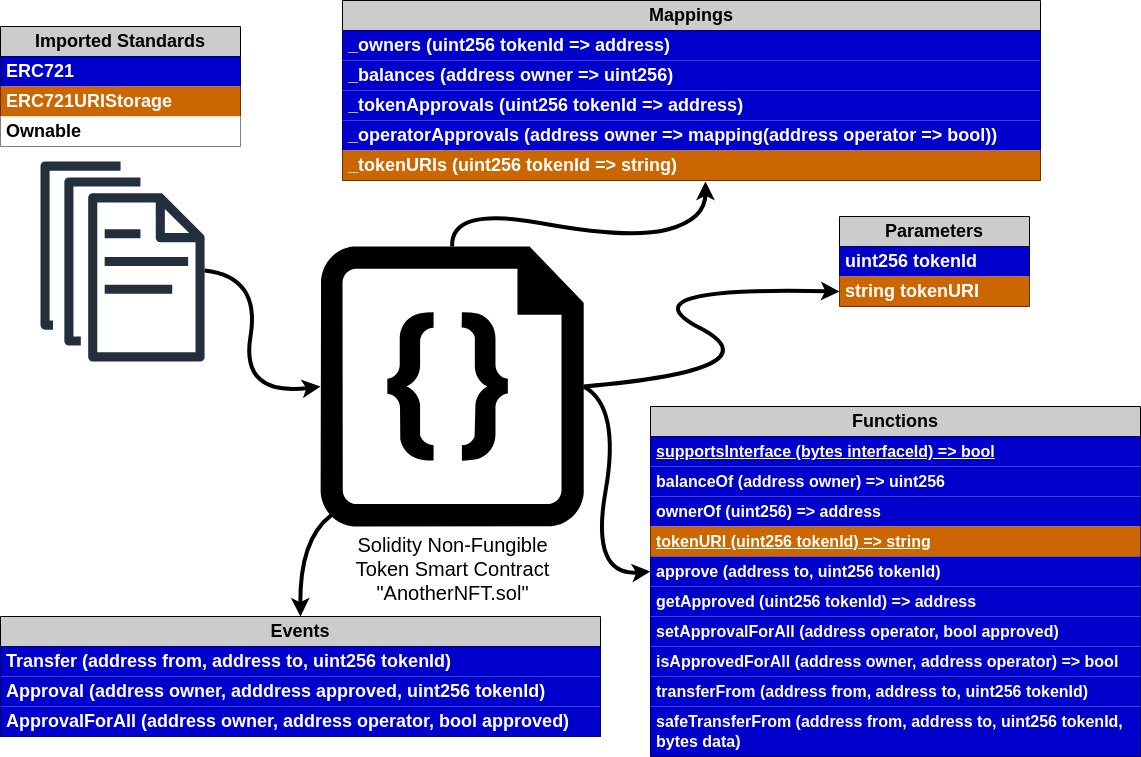
\includegraphics[width=0.85\textwidth]{../Images/04_Solidity_NFT_Contract_Arch.png}
    \caption{General organization of a Solidity NFT minting contract}
    \label{fig:solidity_contract_architecture}
\end{figure}

Fig. \ref{fig:solidity_contract_architecture} references the general architecture followed in the implementation of the example NFT contract. We use a color scheme to identify the parameters, functions, event and mappings (exclusive to Solidity contracts) that are inherited from the standards. In Solidity, importing these interfaces in another contract makes the structures and functions indicated in Fig. \ref{fig:solidity_contract_architecture} available without having to explicitly declare them in the contract. Section \ref{sec:interoperability_functions} goes into more detail about this.

For this purpose, we imported three Solidity interfaces:
\begin{enumerate}
    \item {\textbf{ERC721}} This is the most important standard to implement an Ethereum NFT and that is visible in the amount of functions, parameters, mappings and events inherited from this standard alone.
    \item {\textbf{ERC721URIStorage}} This contract interface is used to establish a more "standardised" way to deal with NFT metadata. It does so by establishing a mapping specific to store that metadata (\textit{\_tokenURIs} mapping), as well as function to retrieve the NFTs metadata.
    \item {\textbf{Ownable}} This interface is used to simplify the establishment and verification of ownership for the contract itself only, hence why no other structures or functions get inherited from this standard. The ownership mechanics for any NFT minted are processed by functions and mappings inherited from the ERC-721 standard. It is possible to write the contract without it, but it makes it unnecessarily complicated.
\end{enumerate}

\subsubsection{Interoperability derived from Standards}
\label{sec:interoperability_functions}
If a user interacts with an ERC-721 compliant Solidity NFT contract, the user can invoke the \textit{balanceOf} function without any need for him/her to check the contract code first to ensure that the function is implemented. In fact, the majority of the cases, this function and others are simply omitted because the interface does not has them marked as \textbf{override}, which means that the implementing contract does not need to have them explicit in its code to have them available for usage. Others, such as \verb|supportsInterface| from the ERC721 standard and \verb|tokenURIs| from the ERC721URIStorage one are marked for overwrite, and as such they need to be explicit in the implementing contract. Overwritten functions are underlined in Fig. \ref{fig:solidity_contract_architecture}. Interface functions marked as \textbf{virtual} can be overwritten.

\subsubsection{Mapping-based Ownership System}
\label{sec:mappings}
Token ownership in the Ethereum network is established by the \verb|\_owners| mapping. When a NFT is minted, a new entry is added to this mapping creating a one-to-one relationship between an account address and a unique \verb|tokenId|. The \verb|tokenId| is unique within the ecosystem defined by the NFT contract. In other words, the NFT is defined by the pair contractName-tokenId.
\par
The NFT metadata is defined through the \verb|_tokenURIs| mapping, but this one is the one inherited by default from the ERC721Storage standard. This standard is not mandatory to implement a NFT in the Ethereum network. Realistically, NFTs can be created without any metadata set, though the usefulness of such construct is limited. Also, a mappings of this type can be added to the NFT contract without importing the ERC721URIStorage, and they can be used to store any kind of string, just like the \verb|_tokenURIs| mapping. But using standards simplifies development and introduces a degree of certainty to other users familiar with them.
\par
The \verb|balances| mapping is self explanatory and the mappings suffixed with "Approvals" are used to delegate token access to other users other than the user. If the user wishes, he/she can use the "approval" functions to set permissions to allow other users to transfer the NFT and execute other owner-exclusive functions. Approval functions change the state of the blockchain, therefore require signed transactions to be executed. Each approval function is owner protected, i.e., they all begun by testing if the address requesting changes to the approval mappings is the owner of the token referred. If that is not the case, the transaction reverts.

\subsubsection{Internal Parameters}
In its most basic form, a standard Ethereum token, i.e., ERC721 compliant token, is defined solely by a \verb|tokenId|, an unsigned 256-bit integer. As mentioned in Sec. \ref{sec:mappings}, NFT metadata is not strictly required and a NFT contract can be implemented without one. The ERC721 standard guarantees solely the existence of the unique token id and, therefore, the uniqueness of the token in the network.

\subsubsection{Events}
Blockchain events are the main information mechanism to detect transaction results and contract changes in the network. Obtaining an output from functions than do not return any values, such as nft mints and token transfers, from any blockchain is quite difficult because one has to look for the correct output from the agglomerate of all the outputs of the various distributed accesses that the blockchain is attending. For a popular and sizeable blockchain, such as Ethereum, that task becomes prohibitive. Events solve this limitation. Event logging is processed differently and these can be indexed, which allows for their fast retrieval and for software tool to pool for these at intervals (event listeners). The ERC721 defines three events by default, one to be emitted whenever a token is transferred(\textit{Transfer}) and two for whenever the approval mappings are modified. These events require arguments to be emitted, which allows for the transmission of specific information with more generalist events. For example, the \textit{Transfer} event, when captured, also indicated the two addresses involved in the transfer and the \verb|tokenId| of the token transferred. The emission of these events is triggered by ERC721 functions, so the whole process is automated and inherited from the contract interface.

\subsection{Functions}
Functions such \textit{balanceOf} and \textit{ownerOf} are self-explanatory and the approval related functions were covered in Sec. \ref{sec:mappings}. The only function inherited from the ERC721URIStorage standard, \textit{tokenURIs} is also quite simple: it receives a \verb|tokenId| as argument and returns the string defined as metadata for the token identified. The \textit{supportsInterface} is used to determine if the contract in question does conform to the ERC721 standard (or any other standards indicated by the contract), and it is not just something the developer is labeling the contract with, but the expected contract interface was not correctly implemented.
\par
Finally, the last functions indicated in Fig. \ref{fig:solidity_contract_architecture} are used to transfer the token to a \verb|to| address. Both functions do what their name suggests, but the "safe" version does additional checks, namely if the receiving address (parameter \verb|to|) is a contract address and, if so, test if the correct NFT receipt was returned from the contract.

% TODO: Mention what was omitted so far from the implementation and that is going to happen in the next "version", namely:
% Token burning
% Changing metadata (v1.0 to v2.0)
% Token approvals (compare how complicated these are when compared with Flow's ownership mechanics)
% Non-blockchain functions, such as encrypt and decrypt data


\end{document}